128. \begin{figure}[ht!]
\center{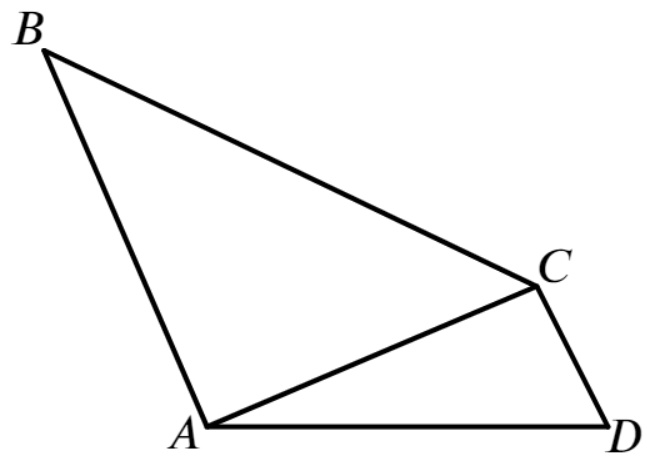
\includegraphics[scale=0.35]{g9-128.png}}
\end{figure}\\
По теореме косинусов для треугольника $ABC$ имеем $AC^2=36+16-2\cdot6\cdot4\cdot\cfrac{5}{6}=12.$ По теореме косинусов для треугольника $ACD$ получим $AC^2=25+64-2\cdot5\cdot8\cdot \cos(\angle D)=12,$ откуда $\cos(\angle D)=\cfrac{77}{80}.$\newpage\noindent
